%% DeepDTA-iBAM -- IEEE Access submission
%%
%% Official IEEE Access author template, downloaded September 26, 2026.
\documentclass{ieeeaccess}

\usepackage{graphicx}
\usepackage{booktabs}
\usepackage{amsmath}
\usepackage{amssymb}
\usepackage{array}
\usepackage{threeparttable}
\usepackage{url}
\usepackage[hidelinks]{hyperref}
\usepackage{cite}
\usepackage{etoolbox}
\usepackage[nopatch=footnote]{microtype}
\usepackage{bm}
% Bold math setup supplied in the official IEEE Access template.
\makeatletter
\AtBeginDocument{\DeclareMathVersion{bold}
\SetSymbolFont{operators}{bold}{T1}{times}{b}{n}
\SetSymbolFont{NewLetters}{bold}{T1}{times}{b}{it}
\SetMathAlphabet{\mathrm}{bold}{T1}{times}{b}{n}
\SetMathAlphabet{\mathit}{bold}{T1}{times}{b}{it}
\SetMathAlphabet{\mathbf}{bold}{T1}{times}{b}{n}
\SetMathAlphabet{\mathtt}{bold}{OT1}{pcr}{b}{n}
\SetSymbolFont{symbols}{bold}{OMS}{cmsy}{b}{n}
\renewcommand\boldmath{\@nomath\boldmath\mathversion{bold}}}
% Publication identifiers have not been assigned at submission.
\patchcmd{\@maketitle}
  {{\vss\doifont Digital Object Identifier\space\@doi\vss}\vspace*{7.4mm}\par}
  {}{}{\PackageError{manuscript}{Could not remove unassigned DOI line}{}}
% Replace the template's zero-width footer boxes with bounded boxes.
\newcommand{\submissionfooter}{%
  \def\@oddfoot{\raisebox{8pt}{\hbox to\textwidth{%
    {\footervolfont Submission manuscript}\hfill{\footerpagefont\thepage}}}}%
  \def\@evenfoot{\raisebox{8pt}{\hbox to\textwidth{%
    {\footerpagefont\thepage}\hfill{\footervolfont Submission manuscript}}}}}
\apptocmd{\ps@titlepage}{\submissionfooter}{}{}
\apptocmd{\ps@headings}{\submissionfooter}{}{}
\pagestyle{headings}
% Reserve space for the template's abstract and keyword bullets.
\newlength{\submissionabstractwidth}
\setlength{\submissionabstractwidth}{\dimexpr\titlewidth-0.5em-1.5mm\relax}
\let\abstractwidth\submissionabstractwidth
% Use available template font shapes for running heads and monospaced paths.
\DeclareFontShape{T1}{formata}{m}{sl}{<->ssub*formata/m/it}{}
\input{t1pcr.fd}
\DeclareFontShape{T1}{pcr}{n}{n}{<->ssub*pcr/m/n}{}
\AtBeginEnvironment{IEEEbiographynophoto}{\phantomsection}
\AtBeginEnvironment{thebibliography}{\raggedright}
\patchcmd{\thebibliography}{\section*{\refname}}
  {\section*{\refname}\phantomsection}{}{}
\makeatother
% Keep natural spacing on pages dominated by floats and between biographies.
\raggedbottom
\setlength{\emergencystretch}{3em}
\patchcmd{\IEEEbiographynophoto}
  {4\baselineskip plus 1fil minus 0\baselineskip}{2\baselineskip}{}{}
\patchcmd{\IEEEbiographynophoto}{\interlinepenalty500}{\interlinepenalty10000}{}{}

\graphicspath{{../results/}{./}}

% Hyphenation exceptions for the recurring compound technical terms; without
% these the narrow IEEE column sets several lines very loose.
\hyphenation{cross-at-ten-tion Re-train-ing ab-la-tion
ab-la-tions in-ter-ac-tion con-cor-dance en-rich-ment fin-ger-print
re-triev-al ar-chi-tec-ture in-ter-pret-abil-ity re-pro-duc-i-bil-ity
che-min-for-mat-ics bio-in-for-mat-ics}

\begin{document}
\bstctlcite{IEEEcontrol}
\history{}
\doi{}
\vol{}
\year{}
\typeout{MANUSCRIPT_TEXT_WIDTH_PT=\the\textwidth}
\typeout{MANUSCRIPT_COLUMN_WIDTH_PT=\the\columnwidth}

%% ------------------------------------------------------------------
%% Title
%% ------------------------------------------------------------------
\title{DeepDTA-iBAM: Cross-Attention Interaction Mapping for Affinity Prediction, Ligand Retrieval, and Analog Generation}
\hypersetup{
  pdftitle={DeepDTA-iBAM: Cross-Attention Interaction Mapping for Affinity Prediction, Ligand Retrieval, and Analog Generation},
  pdfauthor={Kevin Song, John Zhang, Lei Ye, and Jianyi Zhang}}

\author{\uppercase{Kevin Song}\authorrefmark{1},
\uppercase{John Zhang}\authorrefmark{1},
\uppercase{Lei Ye}\authorrefmark{1}, and
\uppercase{Jianyi Zhang}\authorrefmark{1}}
\address[1]{Department of Biomedical Engineering, The University of Alabama
at Birmingham, Birmingham, AL 35294 USA}
\corresp{Corresponding author: Jianyi Zhang (e-mail: jayzhang@uab.edu).}
\tfootnote{This work was supported in part by the National Heart, Lung, and Blood
Institute under Grants U01HL134764, P01HL160476, R01HL131017, and R01HL149137.}

\markboth{Song \headeretal: DeepDTA-iBAM: Cross-Attention Interaction Mapping}%
{Song \headeretal: DeepDTA-iBAM: Cross-Attention Interaction Mapping}

%% ------------------------------------------------------------------
\begin{abstract}
Drug--target affinity models can support screening through affinity scores,
interaction maps, and candidate ranking. We present DeepDTA-iBAM, a
41.5\,M-parameter architecture that integrates these outputs with
protein-conditioned analog generation. A graph encoder represents ligands,
cached protein language-model embeddings represent targets, and bidirectional
cross-attention couples atom and residue tokens for affinity regression,
interaction maps, and retrieval. Analog generation shares the protein adapter
and checkpoint. Retaining the maps adds a measured mean overhead of 1.5\% to
CPU inference time. On a custom random split of the KIBA kinase benchmark, the model achieves a
concordance index of 0.862 and root-mean-square error (RMSE) of 0.452.
At the conventional activity threshold, the area under the receiver operating
characteristic curve (AUROC) is 0.924 and the area under the precision-recall
curve is 0.832, against a positive base rate of 0.214.
Retraining ablations across three seeds do not isolate a dominant component.
Zeroing the trained cross-attention gates raises RMSE by 33\% and reduces
concordance by 0.080. On the docked subset of an assay-defined epidermal growth
factor receptor panel, the model exceeds AutoDock Vina by 0.188 AUROC but trails
fingerprint similarity by 0.156. We identify two benchmark constructions that
prevent valid interpretation and introduce three reporting checks to detect
them. These results support integrated prediction and analysis while
clarifying the limits of interaction-map interpretation and screening performance.
\end{abstract}

\begin{keywords}
\raggedright
Attention mechanisms, benchmark testing, biomedical computing, drug discovery,
machine learning, molecular biophysics, neural network architecture,
performance evaluation.
\end{keywords}

\titlepgskip=-21pt
\maketitle

%% ------------------------------------------------------------------
\section{Introduction}
%% ------------------------------------------------------------------
\PARstart{P}{redicting} how tightly a small molecule binds a protein target
is a core problem in computational drug discovery, and shared datasets such as
KIBA have supported comparisons among successive model generations, from
similarity-based methods through convolutional, graph-based, and
transformer-inspired architectures
\cite{tang2014kiba,he2017simboost,pahikkala2015realistic,ozturk2018deepdta,ozturk2019widedta,karimi2019deepaffinity,tsubaki2019cpi,nguyen2021graphdta,huang2021moltrans,yang2022mgraphdta,huang2022fusiondta,bidgoli2026hmmdta,stepniewska2018pafnucy}.

A single predicted number rarely supports a decision. A project team wants to
know which part of the pocket the prediction rests on, which compounds to order,
and what to make next \cite{schneider2020rethinking}. Meeting those needs with
separate models gives no
guarantee that the explanation corresponds to the prediction it is meant to
explain; meeting them with one model requires an architecture whose internal
representations are shared across tasks by construction.

The original DeepDTA architecture encodes ligand and protein through parallel
convolutional stacks and concatenates the resulting vectors
\cite{ozturk2018deepdta}. Nothing in that design represents which ligand atom
interacts with which residue, so the network emits an affinity scalar and
nothing else. Later work added graph ligand representations
\cite{nguyen2021graphdta,jiang2020dgraphdta,yang2022mgraphdta}, transformer
encoders with substructure interaction maps \cite{huang2021moltrans}, and
learned protein representations with joint attention
\cite{karimi2019deepaffinity}. These approaches motivate integrating predictive
and interpretive outputs within a shared model.

\subsection{Approach}
DeepDTA-iBAM introduces a bidirectional cross-attention
interface between ligand atom tokens and protein residue tokens. The interface
is not an add-on for interpretability: it is the fusion mechanism through which
the affinity head receives information, so the atom-by-residue coupling it
computes contributes directly to the prediction. The fused representation also
supports latent retrieval; analog proposal shares the protein adapter and checkpoint.

Building such a system raises an evaluation problem we treat as part of the
contribution. Affinity prediction has widely used datasets and evaluation
metrics, whereas benchmarks for the secondary capabilities are often assembled
by the authors of each study.
Building those panels ourselves lets us state exactly how each positive class
was defined, and two reveal metrics that are undefined or confounded by the
selection rule.

\subsection{Contributions}
\begin{enumerate}
\item \textbf{A unified multi-task architecture.} A bidirectional
cross-attention interface couples a graph ligand encoder to cached protein
language-model embeddings, so one checkpoint serves affinity regression,
interaction-map extraction, and retrieval through fusion, with analog generation
conditioned on the shared protein adapter (Section~\ref{sec:arch}).

\item \textbf{The cost of collecting interaction maps.} We report
parameter counts, CPU latency, throughput, and how these vary with target length.
Collecting the already-computed maps adds a measured mean overhead of 1.5\%.
Target length is associated with latency and affects batch memory
(Section~\ref{sec:efficiency}).

\item \textbf{An inference-time ablation of the fusion pathway.} Retraining
ablations at three seeds cannot single out any one component. Zeroing the learned
cross-attention gates in the trained checkpoint instead costs 0.080 concordance
index and raises root-mean-square error (RMSE) by a third, demonstrating
dependence on this pathway in the trained model
(Section~\ref{sec:ablation}).

\item \textbf{A direct test of what the interaction maps encode.} We hold the
epidermal growth factor receptor (EGFR) fixed and vary the ligand across
3{,}300 assay-defined actives and
property-matched decoys, then split the attention variance into
ligand-shared and ligand-specific parts. A linear probe then asks how much
predicted affinity and active--decoy labels the maps carry, including for
decoys without reference poses (Section~\ref{sec:maps}).

\item \textbf{Three reporting checks for benchmark validity.} Checks of the base
rate, chance-referenced overlap, and baseline independence identify two
benchmark failures with little additional computation. They distinguish a
repairable benchmark from one that requires rebuilding
(Section~\ref{sec:evalmethod}).
\end{enumerate}

Prior studies of benchmark bias inform this contribution. Benchmarks may
reward memorization when positives are congeneric
\cite{rohrer2009muv,wallach2018memorization}, when uncontrolled
property differences let trivial features carry the score
\cite{sieg2019bias}, or when hidden structure lets a deep network score
well while learning nothing about protein--ligand interaction
\cite{chen2019hiddenbias}. Property-matched decoys are the standard response
\cite{mysinger2012dude,trannguyen2020litpcba}. Our two constructions differ in
kind: one makes the area under the receiver operating characteristic curve
(AUROC) undefined, while the other makes a baseline score
inseparable from the panel's selection rule.

%% ------------------------------------------------------------------
\section{System Architecture}
\label{sec:arch}
%% ------------------------------------------------------------------
DeepDTA-iBAM couples ligand and protein representations through fusion, with
a generation branch conditioned on the protein adapter
(Fig.~\ref{fig:architecture}).

\subsection{Ligand Encoder}
Molecular structures in simplified molecular-input line-entry system (SMILES)
notation are converted to atom--bond graphs with RDKit and encoded by a
multi-head graph attention network \cite{velickovic2018gat} with edge-aware
masking, using 6 layers, 8 heads, and a hidden width of 512. Edge features carry
bond order and ring membership, and each layer applies layer normalization and a
residual connection. Attention pooling produces a graph-level vector alongside
the per-atom token sequence, which is what the fusion stage consumes.

\subsection{Protein Encoder}
Residues are represented by cached embeddings from ESM-C 600M
\cite{esm2024cambrian}, a Cambrian-series protein language model that differs
from ESM-2 \cite{lin2023esm}. Embeddings are computed once per
unique sequence and cached to disk. After cache construction, the language
model need not run during affinity training or inference for cached targets.
A protein adapter projects them to the shared width,
applies a depthwise convolution over sequence position to capture local motifs,
and passes the result through self-attention blocks. Caching is what makes the
system practical: the protein encoder is the most expensive component, and
screening against one target reuses a single cached embedding for every
compound.

\subsection{Bidirectional Cross-Attention Fusion}
The fusion stage distinguishes this architecture. Atom tokens
$A \in \mathbb{R}^{n_a \times d}$ and residue tokens
$R \in \mathbb{R}^{n_r \times d}$ enter three stacked blocks. Here, $n_a$ and
$n_r$ are atom and residue counts, $d$ is the token width, and MHA denotes
multi-head attention. Each block computes attention in both directions,
\begin{equation}
\tilde{A} = \mathrm{MHA}(A, R, R), \qquad
\tilde{R} = \mathrm{MHA}(R, A, A),
\end{equation}
with padding masked on the key side, and updates each stream through a learned
scalar gate,
\begin{equation}
A \leftarrow A + g_a \tilde{A}, \qquad
R \leftarrow R + g_r \tilde{R},
\label{eq:gate}
\end{equation}
followed by a position-wise feed-forward block. The atom-to-residue attention
weights form an $n_a \times n_r$ matrix, the interpretable binding attention map
(iBAM). Averaging it over heads, over the three blocks, and then over a ligand's
real atoms gives a per-residue interaction profile.

Two properties follow from this fusion design. The
map is the coupling used to construct the affinity head's input. It requires
no separate attribution pass, because the weights arise within the forward
pass. Section~\ref{sec:efficiency} measures
what retaining them costs and Section~\ref{sec:maps} tests what they encode,
while the gates in \eqref{eq:gate} being learned scalars gives a clean way to
ablate the pathway at inference (Section~\ref{sec:ablation}).

\subsection{Affinity and Generative Heads}
The affinity head consumes the pooled graph vector, protein vector, and fused
state through a residual multilayer perceptron. Training combines a Huber loss
($\delta = 1.0$), a pairwise ranking term weighted 0.4 after a three-epoch
warmup, and a diffusion auxiliary ramping to 0.02 between epochs 2 and 6. A
target-conditioned denoising diffusion head \cite{ho2020ddpm} operates on the
ligand atom-feature tensor and is reused at inference to propose analogs around
a seed structure. Its conditioning vector is pooled from the protein adapter
before fusion, and generation bypasses the cross-attention blocks.

\begin{figure*}[!t]
\centering
\IfFileExists{../results/fig_architecture.pdf}%
{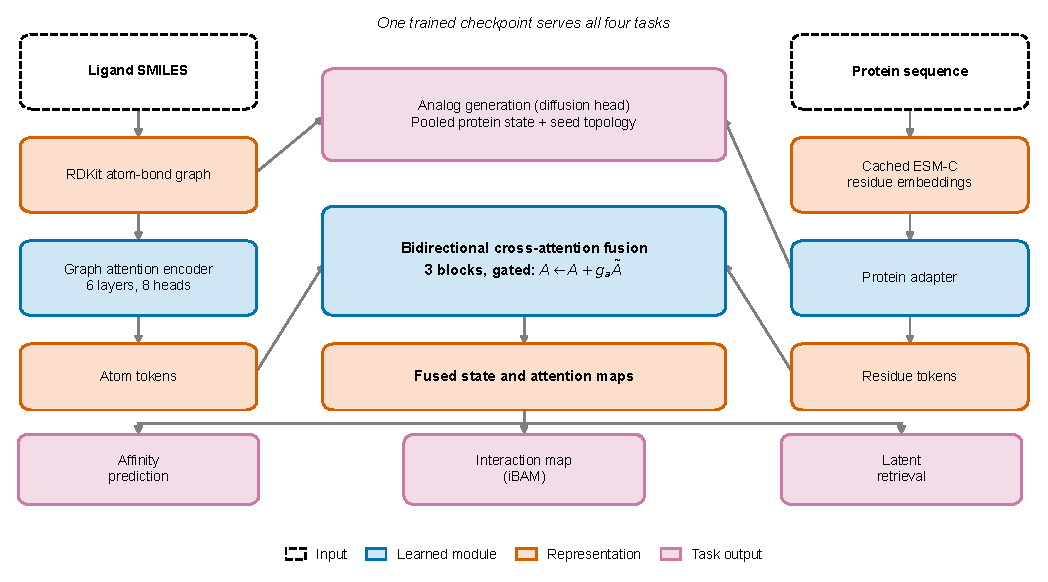
\includegraphics[width=\textwidth]{../results/fig_architecture.pdf}}%
{\fbox{Pending figure}}
\caption{DeepDTA-iBAM architecture. A graph attention encoder turns the ligand
into atom tokens, while cached ESM-C embeddings compressed by a protein adapter
give residue tokens. Three gated bidirectional cross-attention blocks fuse the
two streams for affinity prediction, interaction maps, and latent retrieval.
Generation instead uses the pooled protein-adapter vector and the seed graph.
The affinity head also receives pooled pre-fusion ligand and protein vectors
(omitted here for clarity).
Node class is encoded by fill and border colors, with dashed borders for inputs, as given in the
legend. The atom-by-residue attention matrix reported throughout this paper is
the coupling computed inside the fusion stage, so it is a byproduct of the same
forward pass that produces the affinity prediction rather than a separate
attribution step.}
\label{fig:architecture}
\end{figure*}

%% ------------------------------------------------------------------
\section{Experimental Setup}
\label{sec:setup}
%% ------------------------------------------------------------------

\subsection{Training Data and Checkpoint}
The model was trained on a random 90/5/5 split of KIBA \cite{tang2014kiba},
generated with seed 4221 and termed the standard split here
(106{,}428 training, 5{,}913 validation, and 5{,}913 test pairs), on one GPU.
Evaluation uses the released checkpoint labeled epoch 47 in both its metadata
and optimizer state. A separate training summary ends at epoch 44 and does not
document selection of that checkpoint. Every
analysis uses that single checkpoint, so differences between
experiments reflect evaluation design rather than retraining. The one exception
is the archived component ablation, which aggregates three retraining seeds and so does not reproduce the single-checkpoint values
exactly.

This chemically permissive split differs from published benchmark folds. We therefore
report overlap diagnostics and also evaluate a scaffold split.

\subsection{Structural Panel}
Structural analyses use five kinase co-crystal complexes: 6YOJ (FAK1, ligand
P4N), 4WKQ (EGFR, IRE), 2HYY (ABL1, STI), 1KE6 (CDK2, LS2), and 4RJ3 (CDK2,
3QS), with contacts defined by a 4.5\,\AA{} heavy-atom cutoff throughout.
The panel spans four kinase targets, with two distinct CDK2 complexes.

\subsection{Retrieval Panels}
\label{sec:panels}
Three retrieval panels differ in exactly the respect that determines what each
can measure: how the positive class was defined. Because our claim is that panel
construction determines validity, each rule is stated in full and all are
deterministic in the released code.

\subsubsection{EGFR family panel (similarity-defined)}
Activity records for ChEMBL target CHEMBL203 were retrieved with assay type B,
standard type in $\{K_i, K_d, \mathrm{IC}_{50}\}$, and standard relation
\texttt{=}, requiring a non-null pChEMBL value, the negative base-10 logarithm
of the reported molar potency, and a canonical SMILES string. Relation
operator and measurement type are separate filters and should not be collapsed
into one qualifier: \texttt{=} excludes censored values such as $>$ or $<$,
while the type filter selects which readouts are admitted. $K_i$ and $K_d$
describe inhibition and dissociation, respectively, whereas IC$_{50}$ is a
condition-dependent half-maximal inhibition readout.

Where a pair had several qualifying records, the panel retained the highest
pChEMBL value, ties broken by the lowest nanomolar value, irrespective of
measurement type. Prior work instead imposes a type priority, preferring $K_d$
over $K_i$ and $K_i$ over IC$_{50}$ \cite{valsson2025augmented};
Section~\ref{sec:curation} reports a sensitivity analysis under that priority.

Retained molecules were filtered to pChEMBL $\geq 7.0$ \emph{and} Morgan
extended-connectivity fingerprint (ECFP4, radius 2, 2048 bits)
\cite{rogers2010ecfp} Tanimoto
similarity $\geq 0.40$ to gefitinib (CHEMBL939) or erlotinib (CHEMBL553),
leaving 347 molecules. Tanimoto similarity is the fraction of substructure
features two molecules share, so it runs from 0 for no overlap to 1 for
identical fingerprints. Those two
are the canonical first-generation EGFR inhibitors and 0.40 a conventional
relatedness cutoff; neither is load-bearing, because the defect below follows
from the existence of the similarity filter, not its value.

Six anchors were selected deterministically, not by random seed: the gefitinib
and erlotinib records first, then molecules added greedily, each time
maximizing
\begin{equation}
\min_{j \in S}\left(1 - T(i, j)\right) + 0.03\,p_i,
\end{equation}
where $T$ is Tanimoto similarity to the selected set $S$ and $p_i$ the pChEMBL
value. The remaining 341 became holdout positives.

Decoys came from a local property-filtered lead-like ZINC tranche archive
\cite{irwin2023zinc22}. The first 5{,}000 lines of each tranche file were
scanned and a per-tranche quota of $\lceil 2000/n_{\text{tranches}}\rceil$ was
sampled without replacement under a fixed seed. Any SMILES already in the anchor
or holdout sets was excluded, with deduplication on canonical SMILES throughout.
This gives 2{,}000 decoys and a candidate set of 2{,}341.

\subsubsection{Histamine H1 panel (assay-defined, out of domain)}
Twenty H1 receptor ligands were selected from one ChEMBL page of 1{,}000
assay-type B records, with no standard-type or relation filter. Selection
required pChEMBL $\geq 6.0$ or potency $\leq 1{,}000$\,nM and prioritized a
fixed list of named antihistamines, followed by other named potent candidates
to reach 20 unique SMILES. Candidates were ranked by descending pChEMBL and
ascending nanomolar potency. The released set contains 13 curated-name entries
and 7 fallback entries; clinical phase was recorded when available but was not
an eligibility criterion. Five replicate libraries each contained the same 20 actives and
9{,}980 lead-like compounds drawn from the ZINC bank at five consecutive fixed
seeds, giving 10{,}000 molecules and a positive base rate of 0.002 per library.
No similarity filter was applied at any stage.

\subsubsection{In-domain EGFR panel (assay-defined)}
The Directory of Useful Decoys, Enhanced (DUD-E), supplies EGFR actives
defined by ChEMBL activity and
property-matched decoys \cite{mysinger2012dude}. We sampled 300 actives against
3{,}000 decoys under a fixed seed.

Assay outcome defines the positive class in the second and third panels, while
the first additionally imposes a similarity cutoff. Fingerprint results on
the third panel remain subject to DUD-E's similarity-based decoy selection.

\subsection{Sensitivity to the Activity Consolidation Rule}
\label{sec:curation}
To assess sensitivity to consolidation, we analyzed 19{,}527
cached qualifying CHEMBL203 records, covering 10{,}583 distinct pairs. The mix is
heavily skewed: 18{,}119 records are IC$_{50}$, 875 $K_d$, and 533 $K_i$, and
only 180 pairs, 1.7\%, carry more than one type, so for the large majority the
two rules cannot disagree.

Re-deriving every pair under the $K_d > K_i > \mathrm{IC}_{50}$ priority changes
which record is retained for 64 pairs and the recorded potency for 55, with a
maximum shift of 4.84 log units where a pair carries both a weak binding
constant and a potent functional readout. At the panel's pChEMBL $\geq 7.0$ gate
the retained set moves from 5{,}942 parent IDs to 5{,}928, with 14 dropping out
and none entering, a Jaccard index of 0.998. Applying the similarity cutoff to
this cache gives 756 versus 752 candidates. This larger extraction does not
reproduce the original 347-candidate panel or re-estimate its retrieval metrics.

\subsection{Evaluation Protocol}
The main KIBA evaluation used 2{,}000 bootstrap resamples at a fixed seed; the
earlier evaluation retained in the supplement used 600. Literature benchmark
values are primary-source results under their published splitting protocols
\cite{ozturk2018deepdta,ozturk2019widedta,nguyen2021graphdta,jiang2020dgraphdta,yang2022mgraphdta},
not rerun here, so that comparison is contextual rather than a leaderboard.

Rankers scored on a shared candidate set have correlated errors, so comparing
marginal confidence intervals is not a valid test of their difference;
retrieval comparisons use a paired bootstrap with 10{,}000 resamples at a
fixed seed. The inference-time ablation uses 2{,}000 paired resamples.

For retrieval we report the area under the receiver operating characteristic
curve (AUROC), the area under the precision-recall curve (AUPRC), BEDROC20,
enrichment factors, and recovery at ranked fractions, each beside the positive
base rate.

How the first three behave matters for the rest of the paper. AUROC is the
probability that a randomly chosen active outranks a randomly chosen decoy, and
it is independent of prevalence for fixed class-conditional score distributions.
AUPRC depends on prevalence: the positive fraction is its random-ranking
reference, not a lower bound. BEDROC20 is Boltzmann-enhanced discrimination of
ROC with $\alpha = 20$, emphasizing early retrieval, approximately the first
8\% of the ranked list.

For residue-level contact AUROC we compute an analytic standard error per
complex \cite{hanley1982auroc} and pool by inverse-variance weighting, reporting
fixed-effect and random-effects estimates \cite{dersimonian1986meta}. Derivations are provided in the supplement.

\subsection{Docking Reference}
\label{sec:dockingsetup}
AutoDock Vina 1.2.7 \cite{trott2010vina,eberhardt2021vina} provides an external
structure-based reference. The receptor is chain A of 4WKQ with waters and
cofactors removed, converted to PDBQT with Open Babel at pH 7.4 with Gasteiger
charges, and the search box is centered on the crystallographic gefitinib with
8\,\AA{} padding. Ligands are embedded with RDKit ETKDGv3 at a fixed seed,
optimized with MMFF, and converted with Meeko. Docking used exhaustiveness 8 and
a fixed seed, and scores are negated before computing retrieval metrics because
Vina reports an estimated binding free energy. Using Open Babel rather than the AutoDock
tooling bounds the comparison.

Docking all 3{,}300 candidates requires substantial CPU computation, so the panel was
subsampled. Because retrieval precision is governed by the smaller class and the
panel holds one active per ten decoys, we docked every active and capped the
decoys, drawing them from an order shuffled under a fixed seed. AUROC is
prevalence-independent, but its bootstrap uncertainty depends on class counts;
AUPRC and enrichment factors are reported at the realized prevalence.

All three rankers are evaluated on exactly the docked set. That matters for the
fingerprint baseline, whose released scores are leave-one-out similarities
against all 300 panel actives: scoring a subsample against that full reference
set would hand it evidence the subsample does not contain. We recompute it
within the docked set, which here coincides with the full-panel definition since
every active was docked.

\subsection{Reproducibility}
All analysis code and derived data are released
(\url{https://github.com/kevinmsong/DeepDTA-iBAM}). Every statistic reported
here is supported by scripts and archived outputs in \texttt{analysis/} and
\texttt{results/}, and intermediate artifacts are released so downstream
statistics can be rechecked without rerunning inference. Every random
choice described below, from data splits to bootstrap resampling to decoy
sampling, is seeded; the seed values are set in those scripts rather than
repeated in the text.

A checkpoint audit records file hashes, verifies the epoch-47 optimizer state,
and compares fresh CPU predictions with archived outputs. The incomplete
training history does not establish the checkpoint's original selection
decision. Supplementary audits also recheck atom ordering, candidate curation,
and probe validation while preserving the original artifacts.

The release includes a minimal CPU inference entrypoint. Original weights and
protein caches are not distributed; trained inference requires those assets.
An explicit demonstration with random weights checks tensor flow only.

Inference scripts adjust batch size using the longest target and available
memory, allowing screening runs to adapt to the host. The
checkpoint occupies 166\,MB and the combined graph and protein caches
509\,MB, including 385\,MB of protein embeddings. CPU inference was demonstrated
on a workstation; training used a GPU.

%% ------------------------------------------------------------------
\section{Results}
%% ------------------------------------------------------------------

\subsection{Predictive Accuracy}
\label{sec:accuracy}
On the KIBA test partition the model reaches a concordance index of 0.8625
(95\% bootstrap interval 0.8568 to 0.8681) and RMSE 0.4517 (0.4369 to 0.4673). The
concordance index is the share of pairs the model orders correctly, so 0.5 is
chance and 1.0 is a perfect ranking. It is the standard measure here because
ranking, not the absolute value, is what a screening decision uses.
Binarizing at the conventional activity threshold of 12.1 gives AUROC 0.9240 and
AUPRC 0.8316, which is 3.88 times the positive base rate of 0.2143
(Table~\ref{tab:metrics}).

For context, the original DeepDTA baseline reports 0.863; GraphDTA, DGraphDTA,
and MGraphDTA report 0.891 to 0.904 under their published splitting protocols
\cite{ozturk2018deepdta,nguyen2021graphdta,jiang2020dgraphdta,yang2022mgraphdta};
because those methods were not rerun on our split, these values do not establish
performance parity or a ranking. The architectural contribution is the shared
multi-task interface; its accuracy tradeoff requires a controlled comparison.

Two qualifications matter for deployment. Residuals have a mean bias of
$-0.0095$ with limits of agreement from $-0.895$ to $0.876$, wide enough that a
single predicted value should not drive a commitment to one compound. And all
1{,}587 compounds and 219 targets in the test partition also occur in training,
so this split evaluates unseen pairs of known compounds and targets, without
testing unseen compounds or targets. Under a scaffold split, the same
configuration reaches a concordance index of 0.7615.

\begin{table}[!t]
\caption{Predictive accuracy on the KIBA standard-split test partition.}
\label{tab:metrics}
\centering
\begin{threeparttable}
\IfFileExists{../results/table_benchmark_metrics_expanded.tex}%
{\begin{tabular}{lcc}
\toprule
Metric & Value & 95\% CI \\
\midrule
\multicolumn{3}{l}{\textit{Regression on the KIBA score}} \\
\quad RMSE & 0.4517 & [0.4369, 0.4673] \\
\quad MAE & 0.2950 & -- \\
\quad Pearson $r$ & 0.8741 & -- \\
\quad Spearman $\rho$ & 0.8484 & [0.8373, 0.8588] \\
\quad $R^2$ & 0.7049 & -- \\
\quad Concordance index & 0.8625 & [0.8568, 0.8681] \\
\addlinespace
\multicolumn{3}{l}{\textit{Classification at KIBA $\geq$ 12.1}} \\
\quad Positive base rate & 0.2143 & -- \\
\quad AUROC & 0.9240 & [0.9151, 0.9334] \\
\quad AUPRC & 0.8316 & [0.8139, 0.8503] \\
\quad Balanced accuracy & 0.8587 & -- \\
\quad Matthews correlation & 0.6942 & -- \\
\bottomrule
\end{tabular}
}%
{\fbox{Pending table}}
\begin{tablenotes}[flushleft]\footnotesize\raggedright
\item $n = 5{,}913$ pairs. Lower is better for RMSE and MAE (KIBA-score units);
higher is better for the other performance metrics. The base rate describes
class composition. Intervals are 95\% percentile bootstrap over 2{,}000 resamples;
CI denotes confidence interval. Dashes indicate intervals not reported.
\item The concordance index counts prediction ties as half a concordance and
excludes pairs with equal measured values, the convention the comparison
methods use.
\end{tablenotes}
\end{threeparttable}
\end{table}

\subsection{Component Ablation}
\label{sec:ablation}
Two ablations are reported, because they answer different questions.

\subsubsection{Retraining ablation: no component is resolved}
The archived ablation retrains each variant from scratch with three seeds
(Table~\ref{tab:ablation}). Removing cross-attention, the ranking loss, or the
diffusion head changes standard-split concordance index by at most 0.007 and
scaffold-split by at most 0.009, with every contrast returning $p \geq 0.42$ and
$|d| \leq 0.74$ at $n = 3$, and on the standard split every ablation has a
nominally higher mean than the full configuration.

Estimates from three seeds per variant are too imprecise to attribute
predictive accuracy to an individual component. The multi-task
results establish that the components provide the additional capabilities;
they do not establish an improvement in regression performance.

\subsubsection{Inference-time ablation: what the model relies on}
A different and answerable question is how much the model \emph{as trained}
depends on the cross-attention pathway. Setting the learned gates in
\eqref{eq:gate} to zero removes cross-modal flow while leaving every other weight
exactly as trained, so the degradation is attributable to the pathway rather
than to a different training run reaching a different optimum.

Both gates were initialized at 0.1. After training, gates updating atom tokens
settled at 0.045, 0.040, and 0.061 across the three blocks, while gates updating
residue tokens grew to 0.188, 0.183, and 0.197. Gate magnitudes alone do not
quantify directional importance because the attention updates can differ in scale.

Zeroing them degrades the model substantially (Table~\ref{tab:ablation_inf}). On
1{,}200 held-out KIBA pairs the intact checkpoint reaches concordance index
0.8613 and RMSE 0.4475, consistent with the full-test estimates. With the gates
off, concordance falls to 0.7809 and RMSE rises to 0.5948. The bootstrap mean intact-minus-zeroed RMSE
difference is $-0.148$ KIBA units (95\% CI $-0.190$ to $-0.107$),
corresponding to a 33\% increase in RMSE, with
concordance index down 0.080. Halving the gates reduces concordance index by
0.0105, with the interval for the RMSE difference spanning zero.

So the trained model does depend on the fusion pathway even though the
retraining ablation resolved nothing. These are not contradictory: a retrained
model could compensate through its remaining capacity, whereas this one never
had that opportunity. The inference-time result measures sensitivity to removing the pathway in this
checkpoint. Resampling individual pairs does not capture training variability
or dependence among pairs sharing compounds or targets.

\begin{table}[!t]
\caption{Inference-time ablation of the cross-attention pathway, on 1{,}200
held-out KIBA pairs.}
\label{tab:ablation_inf}
\centering
\begin{tabular}{lccc}
\toprule
Condition & Concordance & RMSE & Pearson $r$ \\
\midrule
Intact                  & 0.8613 & 0.4475 & 0.8760 \\
Gates halved            & 0.8508 & 0.4521 & 0.8641 \\
Gates zeroed            & 0.7809 & 0.5948 & 0.7355 \\
\bottomrule
\end{tabular}
\end{table}

\begin{table}[!t]
\caption{Retraining ablation: concordance index across three independently
retrained seeds per variant.}
\label{tab:ablation}
\centering
\begin{threeparttable}
\begin{tabular}{llcr}
\toprule
Split & Variant & \shortstack{Concordance\\(mean $\pm$ SD)} & $p$ \\
\midrule
Standard & Full model         & 0.8562 $\pm$ 0.0098 & -- \\
         & No cross-attention & 0.8596 $\pm$ 0.0055 & 0.63 \\
         & No ranking loss    & 0.8634 $\pm$ 0.0096 & 0.42 \\
         & No diffusion head  & 0.8582 $\pm$ 0.0057 & 0.78 \\
         & Backbone only      & 0.8633 $\pm$ 0.0113 & 0.46 \\
\midrule
Scaffold & Full model         & 0.7615 $\pm$ 0.0308 & -- \\
         & No cross-attention & 0.7529 $\pm$ 0.0154 & 0.70 \\
         & No ranking loss    & 0.7658 $\pm$ 0.0302 & 0.87 \\
         & No diffusion head  & 0.7691 $\pm$ 0.0243 & 0.75 \\
         & Backbone only      & 0.7669 $\pm$ 0.0196 & 0.81 \\
\bottomrule
\end{tabular}
\begin{tablenotes}[flushleft]\footnotesize\raggedright
\item SD denotes standard deviation.
$p$ is a two-sided Welch two-sample test of each variant against the full
configuration on the same split. At $n = 3$ the panel cannot separate
differences of this size, so these rows bound what the design can show rather
than attributing accuracy to any component.
\end{tablenotes}
\end{threeparttable}
\end{table}

\subsection{Efficiency and Scalability}
\label{sec:efficiency}
We measured the cost of retaining the interaction map from the prediction's
forward pass. All
timings are single-process CPU numbers on an 11th-generation Intel Core machine
using 8 threads, the relevant setting for a screening deployment without
accelerators; the checkpoint itself was trained on GPU.

\subsubsection{Where the parameters are}
The model has 41.5\,M parameters (Fig.~\ref{fig:efficiency}a): cross-attention
fusion 19.7\,M (47.4\%), protein adapter 13.3\,M (32.1\%), affinity head 5.8\,M
(13.9\%), ligand graph encoder 2.0\,M (4.9\%), and diffusion head 0.70\,M (1.7\%).
The interaction map is therefore not free in parameters, since fusion is the
single largest component. What it buys is that those parameters are spent on the
computation producing the prediction, not on a parallel explanation pathway.

\subsubsection{Measured map-collection overhead}
Table~\ref{tab:efficiency} compares per-pair latency with and without
collecting the attention maps at each batch size. Both paths compute the
attention weights; this comparison measures their collection overhead. The difference averages
$+1.5\%$, ranging from $-1.4\%$ to $+6.6\%$. These descriptive timings suggest
small collection overhead; repeated timing runs would be needed to estimate
its uncertainty.

\subsubsection{Batch size and target length}
Throughput is highest at one pair per batch, 204\,ms per pair, and falls
monotonically as the batch grows: 217\,ms at 4 pairs, 232\,ms at 8, 295\,ms at 16,
and 459\,ms at 32 (Fig.~\ref{fig:efficiency}b). At 64 pairs the run exhausts
memory, requesting a single 34.9\,GB allocation on a 64\,GB machine.

Padding can contribute because the protein adapter's self-attention scales
with batch size and the square of the longest sequence length. However, the
loader sorts by length and excludes two warmup batches per setting, leaving
different timed subsets (254 to 192 pairs). This sweep therefore does not
isolate batch size from target composition. Within the single-pair run, a
single-pair regression over targets from 292 to 4{,}128 residues gives 0.477\,ms
per residue with Pearson $r = 0.919$ ($n = 254$), while ligand size shows
little linear association with latency ($r = -0.03$).

These measurements motivate testing small, length-grouped batches and
choosing batch size for the target lengths and available memory.

\subsubsection{Cached embeddings make screening practical}
The timing sample used cached ESM-C embeddings for 132 unique targets,
and the protein-embedding file occupies 385\,MB; the combined graph and
protein cache occupies 509\,MB. Reusing these embeddings avoids running the
protein language model for each candidate. The reported 210\,ms per pair
excludes initial embedding computation.

\begin{table}[!t]
\caption{CPU inference latency per pair, with and without collecting the
interaction maps.}
\label{tab:efficiency}
\centering
\begin{tabular}{rccr}
\toprule
Pairs per & Scores only & Maps collected & Difference \\
batch & (ms/pair) & (ms/pair) & \\
\midrule
1  & 204.0 & 209.6 & $+2.7\%$ \\
4  & 216.6 & 213.6 & $-1.4\%$ \\
8  & 232.3 & 233.7 & $+0.6\%$ \\
16 & 295.5 & 292.6 & $-1.0\%$ \\
32 & 458.9 & 489.2 & $+6.6\%$ \\
64 & \multicolumn{3}{c}{out of memory (34.9\,GB requested)} \\
\bottomrule
\end{tabular}
\end{table}

\begin{figure*}[!t]
\centering
\IfFileExists{../results/fig_efficiency.pdf}%
{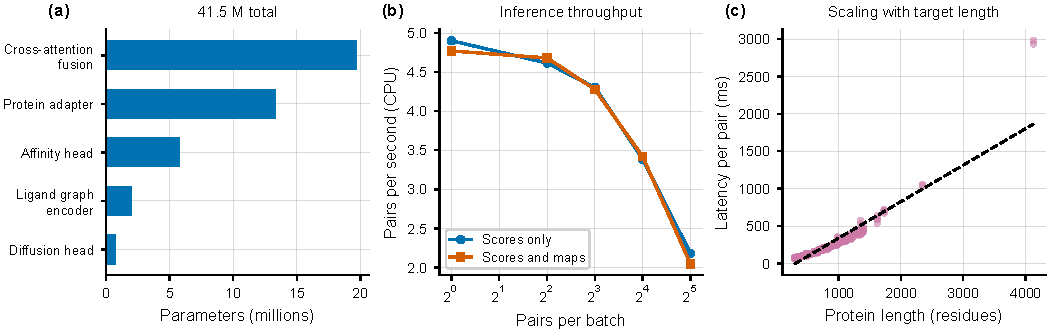
\includegraphics[width=\textwidth]{../results/fig_efficiency.pdf}}%
{\fbox{Pending figure}}
\caption{Cost profile of the inference path, measured on CPU.
(a) Parameters by module; the cross-attention fusion that produces the
interaction maps is the largest single component at 47.4\% of 41.5\,M
parameters. (b) Throughput against pairs per batch, with and without
collecting the attention maps. The curves are similar, with an average
latency difference of 1.5\%. Timed subsets differ across batch sizes because
two warmup batches are excluded from each length-sorted run. (c) Single-pair
latency against target length, a major determinant of time and memory.}
\label{fig:efficiency}
\end{figure*}

\subsection{What the Interaction Maps Encode}
\label{sec:maps}
Fig.~\ref{fig:ibam} shows what one of these maps looks like, and the rest of
this section measures what such a map does and does not carry.

Contact benchmarks scored against a crystal pose cannot assess compounds without
reference poses. The in-domain EGFR panel includes decoys that are presumed
inactive without experimental confirmation. The target is
fixed, the ligand varies over 300 actives and 3{,}000 property-matched decoys,
and the model emits a map for every one. We extracted the per-residue profile
for all 3{,}300 candidates; this rerun reproduced the released affinity scores
to a correlation of 1.000000.

\begin{figure*}[!t]
\centering
\IfFileExists{../results/fig_ibam_map.pdf}%
{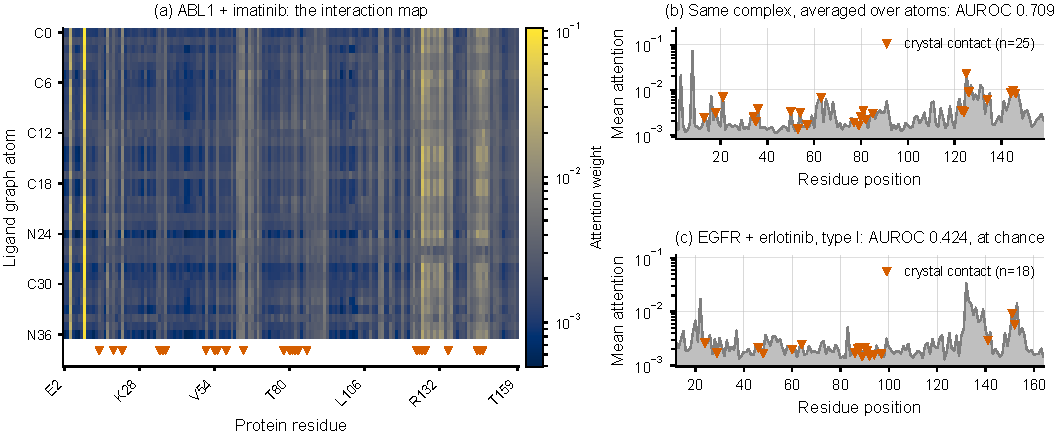
\includegraphics[width=\textwidth]{../results/fig_ibam_map.pdf}}%
{\fbox{Pending figure}}
\caption{Attention maps and their agreement with crystallographic contacts.
(a) The atom-by-residue attention matrix for ABL1 with imatinib (PDB 2HYY),
taken from the same forward pass that produces the affinity prediction. Rows are
ligand graph atoms, columns residues, and the triangles below mark the 25
residues within 4.5\,\AA{} of the ligand in the crystal. Color is on a log scale
because the weights span more than two decades. The pattern is almost entirely
vertical, meaning every ligand atom attends to nearly the same residues, and the
brightest bands fall in the contact-rich region.
(b) The corresponding released per-residue profile, obtained by averaging
attention over atoms, at a residue contact AUROC of 0.709.
(c) The per-residue profile for EGFR with gefitinib, whose interval
includes chance. Attention localizes in two of the five complexes
(Fig.~\ref{fig:forest}), so (a) is the better case rather than the typical one.
Panels show contact-region windows; AUROCs use all evaluated residues.
The matrix and released profiles come from separate inference runs.}
\label{fig:ibam}
\end{figure*}

\subsubsection{Most of the map is shared across the tested ligands}
Decomposing the variance of the 3{,}300 by 1{,}210 profile matrix separates the
panel-mean residue profile from the deviations specific to each tested ligand. The
residue main effect accounts for 92.7\% of the variance and the
ligand-by-residue interaction for 7.3\%; the ligand main effect is zero by
construction, because each profile is a distribution over residues
(Fig.~\ref{fig:maps}a). Profiles correlate with the panel mean at 0.968 on
average and with each other at 0.938 (Fig.~\ref{fig:maps}b).

The practical reading is that an interaction map shown for a single compound is
mostly a target-associated residue profile. Presenting one as an explanation specific to
that compound overstates what distinguishes it from any other ligand, a caution
that applies to attention heatmaps generally
\cite{jimenezluna2020xai,jain2019attention,wiegreffe2019attention}.

\subsubsection{The remaining 7.3\% carries signal}
The residual profiles retain predictive information. Features are standardized
per residue, so the shared residue component is removed before fitting and
what follows uses only the ligand-specific part.

Logistic probes used shuffled stratified five-fold cross-validation with fixed
L2 regularization ($C = 0.1$), balanced class weights, and standardization fitted
within each training fold. Ridge regression used shuffled five-fold outer
cross-validation, selecting among penalties 1, 10, 100, and 1{,}000 through
five-fold inner cross-validation restricted to each outer training fold.
Ridge regression from the profile to predicted affinity reaches a
cross-validated $R^2$ of 0.321, against $-0.029$ for a shuffled target. A linear
readout of the map therefore recovers part of the model's predicted affinity.

The active versus decoy comparison is shown in Fig.~\ref{fig:maps}c. A
cross-validated logistic probe on the profile separates actives from decoys at
AUROC 0.984, against 0.909 for a probe on ten bulk physicochemical descriptors
and 0.499 under shuffled labels. A profile might merely encode ligand size, so
we residualized it on those descriptors by fitting the descriptor-to-profile
regression within each outer training fold and applying it to held-out candidates.
The resulting AUROC is 0.963, suggesting label-associated information beyond
this linear descriptor adjustment. These random candidate folds do not test
generalization to new chemical series or targets. The analysis uses a fixed
checkpoint and one set of folds; the shuffled controls use one fixed permutation.

One comparison must not be drawn from these numbers. The probes are supervised
and fitted on this panel, whereas the model's own affinity score (AUROC 0.839)
was not fitted on panel labels. The fingerprint baseline (0.992) uses known
active references without fitting a classifier. These different uses of labels
prevent a direct performance comparison. The probes suggest that the maps
contain information associated with active--decoy labels, subject to DUD-E's
decoy-selection bias.

\subsubsection{Agreement with crystallographic contacts}
Residue-level attention agrees with crystallographic contacts to varying degrees
across the five complexes (Fig.~\ref{fig:forest}). ABL1 with imatinib reaches
AUROC 0.709 (95\% CI 0.591 to 0.827) and CDK2--3QS 0.702 (0.568 to 0.837), both
excluding chance, whereas CDK2--LS2, EGFR, and FAK1 do not. The panel is strongly
heterogeneous ($Q = 15.5$ on 4 df, $I^2 = 74\%$), so the random-effects estimate
of 0.585 (0.470 to 0.701, $p = 0.15$) is the defensible summary, not the
fixed-effect 0.586.

This small panel does not establish a shared localization effect or explain
the observed variation. A larger panel with
verified structural annotations is needed.

\begin{figure}[!t]
\centering
\IfFileExists{../results/fig_localization_forest.pdf}%
{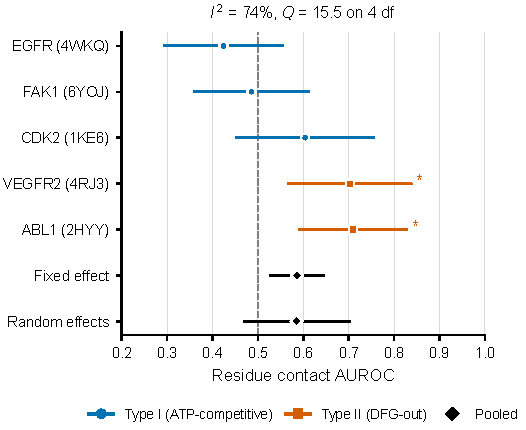
\includegraphics[width=\columnwidth]{../results/fig_localization_forest.pdf}}%
{\fbox{Pending figure}}
\caption{Residue contact AUROC by complex, with analytic Hanley--McNeil
95\% confidence intervals computed from the 250 to 300 residues within each complex rather than
treating each complex as one observation. Asterisks mark intervals excluding
chance. Diamonds give fixed-effect and
random-effects pooled estimates. The wider random-effects interval reflects
between-complex heterogeneity; individual intervals are unadjusted for multiplicity.}
\label{fig:forest}
\end{figure}

\begin{figure*}[!t]
\centering
\IfFileExists{../results/fig_interaction_content.pdf}%
{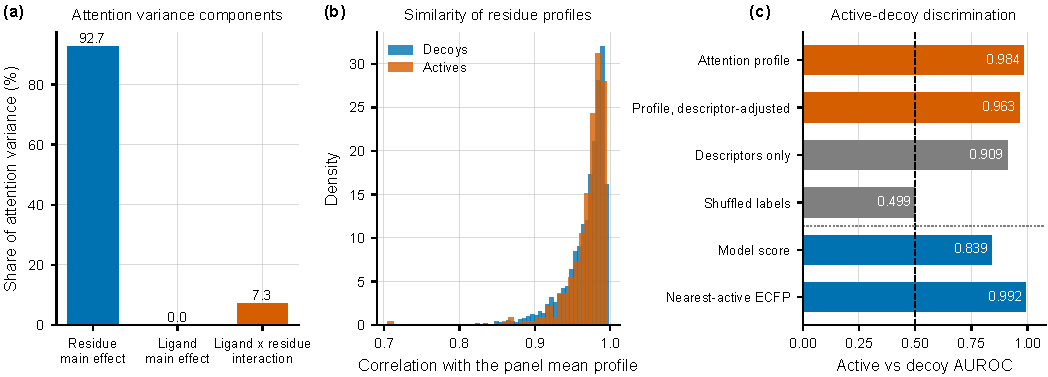
\includegraphics[width=\textwidth]{../results/fig_interaction_content.pdf}}%
{\fbox{Pending figure}}
\caption{What the interaction maps encode, measured on 300 assay-defined EGFR
actives and 3{,}000 property-matched decoys against a fixed target.
(a) Variance decomposition of the ligand-by-residue attention matrix: 92.7\% of
the variation is the residue main effect shared across the tested ligands, and
7.3\% is the ligand-specific interaction. (b) Each ligand's profile correlates
with the panel mean profile at 0.968 on average, so a map shown for one compound
is largely target-associated. (c) Active versus decoy AUROC. The first
four bars are supervised probes fitted by cross-validation; the last two are
rankers without panel-specific classifier fitting and are not directly comparable
to the probes; the fingerprint ranker uses known active references. A probe on the
profile beats a probe on bulk descriptors, and still does so after the profile
is residualized on those descriptors. Standardization and descriptor
residualization were fitted within each training fold; estimates use combined
out-of-fold predictions under random candidate splits.}
\label{fig:maps}
\end{figure*}

\subsection{Retrieval Validation}
\label{sec:retrieval}
Library prioritization is the application most often claimed for a drug--target
affinity model, so it deserves the strictest test. We evaluate it only on the
two panels whose positives are assay-defined, using a ligand-similarity
baseline on both and AutoDock Vina on EGFR.

\subsubsection{Out of domain}
The similarity baseline scores each candidate by its fingerprint resemblance to
the nearest known active, with that candidate itself excluded when it is one of
them. On the H1 panel this baseline reached AUROC 0.996 and
AUPRC 0.806, recovering 17 of 20 actives within the top 1\% and all 20 within
the top 5\%, while DeepDTA-iBAM reached 0.667 $\pm$ 0.008 and
0.021 $\pm$ 0.018 (mean $\pm$ SD across five libraries), recovering 14\%
within the top 10\%. H1 is a G-protein-coupled receptor and the model was trained on
kinase-dominated data, so this measures transfer rather than performance on the
model's own family. The small replicate variance shows the weak signal is
reproducible across background libraries rather than an artifact of one draw.

\subsubsection{In domain, against similarity and docking}
The in-domain EGFR panel provides a complementary test: assay-defined actives,
property-matched decoys, and a target from the model's own family. Across all
3{,}300 candidates the fingerprint baseline reached AUROC 0.992 and recovered
97.0\% of actives within the top 10\%, against 0.839 and 60.7\% for the model,
a paired model-minus-fingerprint difference of $-0.153$ (95\% CI $-0.184$ to $-0.125$).

Docking places that gap on an external scale (Table~\ref{tab:docking},
Fig.~\ref{fig:docking}a). On the docked set of all 300 actives and 460 decoys,
all of which prepared successfully, Vina reached AUROC 0.648, the model 0.836,
and the fingerprint baseline 0.992. Both paired bootstraps resolve: the model
leads Vina by 0.188 AUROC (95\% CI $+0.139$ to $+0.237$) and trails the
fingerprint baseline by 0.156 ($+0.125$ to $+0.189$), the latter reproducing the
full-panel ordering and giving a similar margin.

These comparisons have distinct limitations. Receptor preparation used Open
Babel, and Vina used one rigid receptor conformation. The gap behind the fingerprint baseline holds on two
target panels, but DUD-E requires decoys topologically dissimilar to its
actives, which favors fingerprint methods
\cite{mysinger2012dude,chen2019hiddenbias,wallach2018memorization}. The 0.156
gap may therefore overstate the difference on a panel without this selection bias.

\begin{table*}[!t]
\caption{In-domain EGFR retrieval on the docked set: 300 assay-defined actives
and 460 property-matched decoys.}
\label{tab:docking}
\centering
\footnotesize
\IfFileExists{../results/docking_revalidated/table_docking_retrieval.tex}%
{\begin{tabular}{lcccccc}
\toprule
Ranker & AUROC & AUPRC & BEDROC20 & EF 1\% & EF 5\% & Rec.\ 10\% \\
\midrule
AutoDock Vina & 0.648 & 0.493 & 0.463 & 0.95 & 1.07 & 0.129 \\
DeepDTA-iBAM & 0.836 & 0.836 & 0.976 & 2.53 & 2.47 & 0.250 \\
Nearest-active ECFP & 0.992 & 0.992 & 1.000 & 2.53 & 2.53 & 0.253 \\
\bottomrule
\end{tabular}
}%
{\fbox{Pending table}}
\vspace{3pt}
\begin{minipage}{0.85\textwidth}\footnotesize
Higher is better throughout. Vina reports an estimated binding free energy, so its score is
negated before ranking. AUROC is insensitive to prevalence alone, but all
metrics may change with candidate composition. AUPRC and enrichment factors
also depend on prevalence and are reported at the realized 39.5\% active fraction, so
they cannot be compared with enrichment figures quoted for the full 1:10 panel.
EF denotes enrichment factor at the indicated ranked fraction; Rec.\ 10\%
is the fraction of actives recovered in the top 10\%. EF, recovery, and BEDROC
average over all orderings within tied-score groups.
\end{minipage}
\end{table*}

\begin{figure*}[!t]
\centering
\IfFileExists{../results/fig_docking.pdf}%
{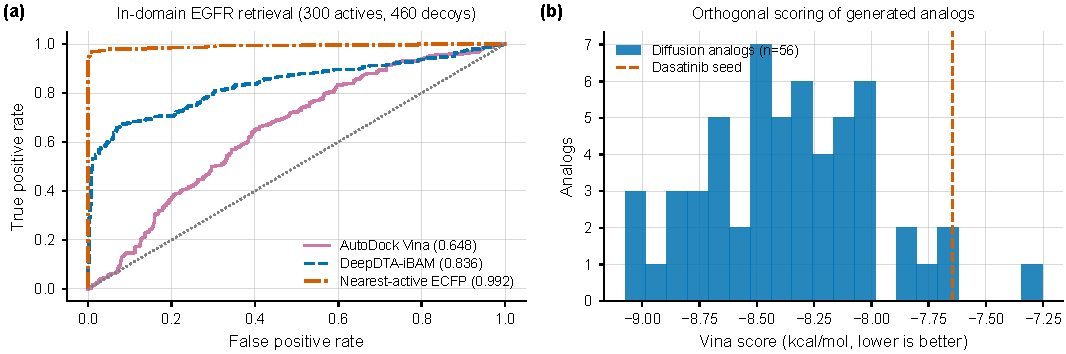
\includegraphics[width=\textwidth]{../results/fig_docking.pdf}}%
{\fbox{Pending figure}}
\caption{An external structure-based reference for both secondary capabilities.
(a) Retrieval on the in-domain EGFR panel. The learned scorer outranks AutoDock
Vina, and a nearest-active fingerprint search outranks both. Vina used Open
Babel receptor preparation and a single rigid conformation, which bounds the
first comparison. Panel (a) shows ROC curves for 300 actives and 460 decoys.
(b) Vina scores for the 56 audited diffusion analogs that
could be prepared, against the dasatinib seed. Lower is better. The analogs
include 55 with lower scores than the seed under a scorer that played no part in
generating them.}
\label{fig:docking}
\end{figure*}

Similarity search provides a strong reference on these panels when known
actives are available. The learned scorer warrants further evaluation when
reference actives are unavailable or when interaction maps and a shared latent
representation are also needed.

\subsection{Local Design}
\label{sec:generation}
Under EGFR conditioning from dasatinib the diffusion head returned 100 unique
valid molecules within 4{,}000 decode attempts, against 100 for fragment swaps
and 40 for random atom edits, so it has a yield advantage over random edits
only.

Diffusion proposals have a median
fingerprint similarity of 0.14 to the seed, against 0.59 for fragment swaps and
0.84 for random edits (Fig.~\ref{fig:generation}a), giving them the lowest
median similarity among the three generators. Fragment swaps score better on
all four reported chemical heuristics (Fig.~\ref{fig:generation}b):
quantitative estimate of drug-likeness (QED, 0.562 versus 0.402), synthetic accessibility (2.93
versus 4.03), Lipinski pass rate (0.94 versus 0.44), and alert-free rate (0.74
versus 0.38)
\cite{bickerton2012qed,ertl2009sa,lipinski2001ro5,brown2019guacamol}.

\begin{figure*}[!t]
\centering
\IfFileExists{../results/fig_generation.pdf}%
{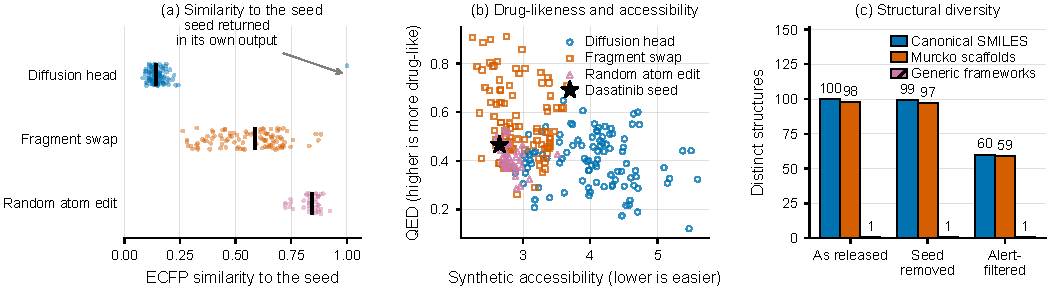
\includegraphics[width=\textwidth]{../results/fig_generation.pdf}}%
{\fbox{Pending figure}}
\caption{What the analog-generation head does, on 100 diffusion proposals, 100
fragment swaps, and 40 random atom edits conditioned on EGFR from a dasatinib
seed. (a) Fingerprint similarity of each proposal to the seed, with the median
marked. Diffusion proposals have the lowest median similarity; the single
proposal at 1.0 is the seed, returned in its own
output. (b) Drug-likeness against synthetic accessibility for the same
molecules. Diffusion proposals have lower QED and higher synthetic accessibility
scores than fragment swaps on average. (c) Distinct structures through the audit under three definitions.
Canonical SMILES and Bemis--Murcko scaffolds track the set size, which reads as
near-complete diversity, but generic frameworks, the same skeletons with atom
types and bond orders erased, stay at one throughout. The head varies
substituents widely around a single fixed skeleton.}
\label{fig:generation}
\end{figure*}

Diffusion did give the highest mean predicted affinity, 11.289 against 11.196
for random edits and 11.079 for fragment swaps, with the returned seed at 11.269
in the same candidate-scoring pass. That
cannot establish superiority: every candidate is rescored by the checkpoint that
produced the diffusion proposals, so it measures agreement between a generator
and its own critic, and both margins are below the held-out RMSE.

Auditing the set molecule by molecule found two problems the aggregate
statistics hid; the full audit is in the supplement. One of the 100 molecules is
dasatinib itself, so the seed was retained in its own output. Another 39 of the
remaining 99 carry motifs that pass RDKit sanitization but are not credible
follow-up candidates under the audit criteria, leaving 60 analogs.

Figure~\ref{fig:top_analogs} shows the seed and the five highest-scoring
analogs among these 60, ordered by their saved predictions. Predicted KIBA
scores span 11.855 to 11.993, compared with 11.269 for the seed in the same
scoring pass. All remain below the conventional KIBA activity threshold of
12.1. Four fail the reported Lipinski screen, and the highest-scoring
analog also triggers a PAINS/BRENK alert. These examples illustrate why model
ranking must be considered alongside chemical filters. Potential stereocenters
are unspecified in their SMILES; the saved docking scores refer to
the prepared structures and do not compare all possible stereoisomers.

\begin{figure*}[!t]
\centering
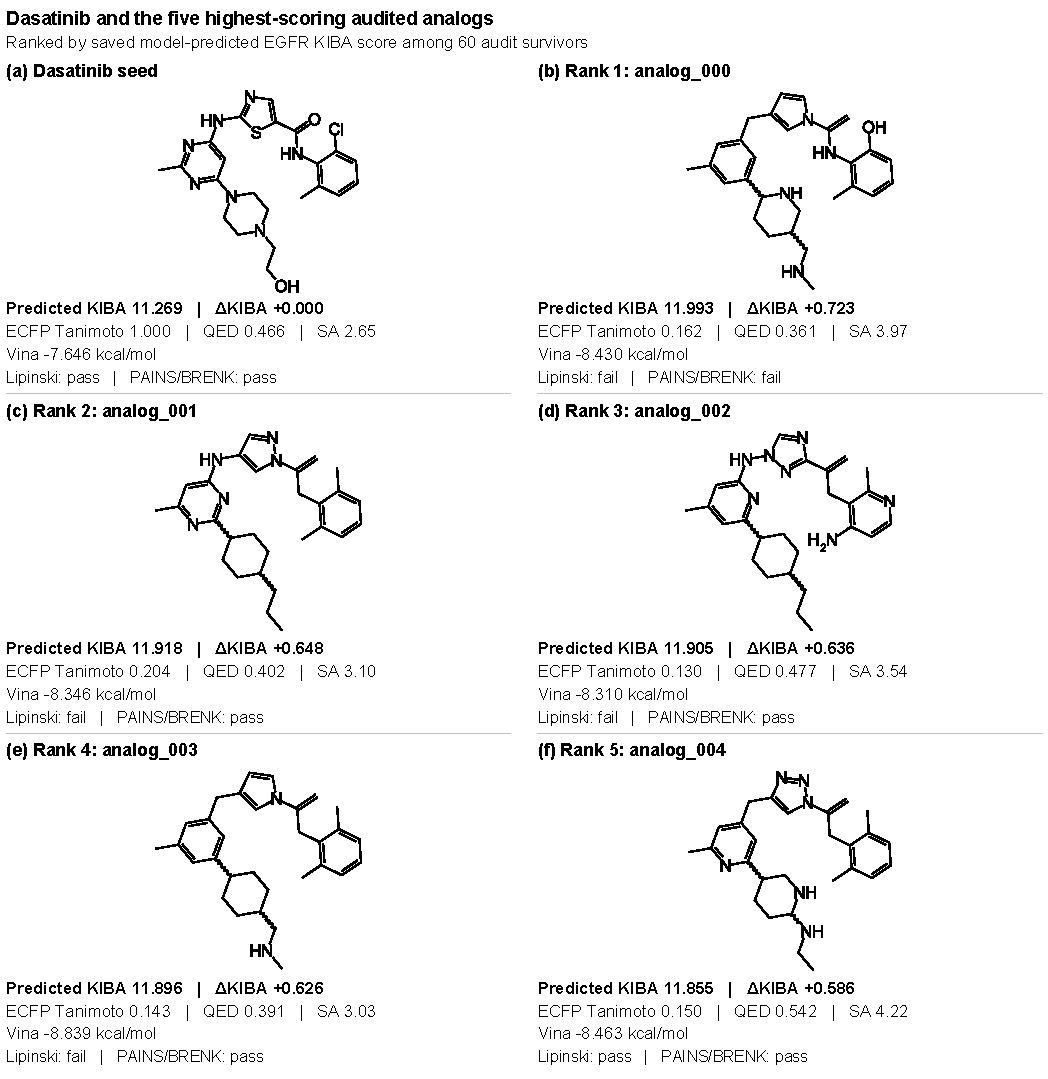
\includegraphics[width=\textwidth]{../results/fig_top_analogs.pdf}
\caption{Dasatinib seed and the five highest-ranked EGFR-conditioned diffusion
analogs among 60 nonseed candidates retained by the four-motif audit.
Ranking uses saved predicted KIBA scores; $\Delta$KIBA is the difference from
the seed scored in the same pass. ECFP Tanimoto compares radius-2, 2{,}048-bit
fingerprints with the seed. Higher QED indicates greater drug-likeness;
lower synthetic accessibility (SA) scores indicate easier predicted synthesis.
Vina values are archived docking scores, with lower values preferred.
Lipinski and PAINS/BRENK screening flags are separate from the four-motif
audit. Wavy bonds indicate unspecified stereochemistry. Predictions,
heuristics, and docking scores do not establish potency or synthetic feasibility.}
\label{fig:top_analogs}
\end{figure*}

The second problem is the more consequential (Fig.~\ref{fig:generation}c).
Uniqueness had been assessed by canonical SMILES, and on that criterion all 100
molecules are distinct, with 98 distinct Bemis--Murcko scaffolds, the ring
systems and the linkers between them. That reads as near-complete scaffold
diversity. Yet all 100 share a
\emph{single} generic framework, the same skeleton with every atom type erased,
and it is dasatinib's \cite{bemis1996frameworks}. This follows mechanically from
a decoder that holds bond topology fixed, so it is not a malfunction, but the
head is enumerating substitutions around one skeleton rather than exploring
chemical space. Diversity should be reported by generic framework, not by
counting SMILES.

Docking supplies the missing scorer (Fig.~\ref{fig:docking}b). Of those 60
analogs 56 could be prepared; 4 failed charge assignment, indicating remaining
preparation limitations. The 56 scored a mean of $-8.364$\,kcal/mol against $-7.646$ for the
seed, with 55 of 56 better than it.

Read this narrowly. Vina scores track molecular size and these are substitutions
on the seed's own skeleton, so a systematic shift is unsurprising. The result
provides a comparison independent of the model's affinity head, with lower
scores than the starting structure for 55 analogs. It does not establish
improved potency or synthetic feasibility.

%% ------------------------------------------------------------------
\section{Evaluation Methodology}
\label{sec:evalmethod}
%% ------------------------------------------------------------------
Building the panels ourselves exposed two constructions that prevent valid
interpretation. The remedy depends on the failure: a single-class AUROC needs
different labels, while matching on similarity requires overlapping class supports.

\subsection{Base-Rate Saturation}
In the evaluated kinase complexes essentially every ligand heavy atom lies
within 4.5\,\AA{} of protein. Across our five complexes the atom contact counts
were 26 of 27, 37 of 37, 29 of 29, 31 of 31, and 34 of 34: every ligand atom was
a contact in four of the five, and 96.3\% in the fifth
(Fig.~\ref{fig:validity}a).

These contact labels describe the reference structures and do not depend on
model predictions. At the chosen 4.5\,\AA{} cutoff, the atom-level labels are
saturated in this panel.

Two consequences follow mechanically. Contact AUROC is undefined when every
label is the same, so whatever a results table prints there is a software
artifact. And top-$k$ overlap, where $k$ is the number of true contacts, has a
chance expectation of exactly $k/n$, the contact base rate: at a base rate of
0.993 the observed 0.992 is an excess over chance of $-0.0003$ (95\% CI
$-0.001$ to $+0.001$). Without the base rate beside it, the raw overlap reads as
strong attribution and a fallback AUROC as inverted attribution, although
these summaries provide little evidence of attribution.

The residue-level half remains well posed, with contact base rates of 5.7\% to
9.5\%, which is exactly the contrast the base rate makes visible. At the atom
level, informative evaluation requires labels or metrics that distinguish
atoms, such as graded buried surface area or a panel with more solvent-exposed
ligand atoms.

\subsection{Selection-Rule Circularity}
The EGFR family panel of Section~\ref{sec:panels} required Tanimoto similarity
$\geq 0.40$ to gefitinib or erlotinib, and the anchors came from that same
filtered family, so all 347 molecules satisfy the constraint by construction.

The consequence is stronger than leakage. Positives span 0.400 to 0.904 in
nearest-anchor similarity and decoys span 0.054 to 0.233, so the largest decoy
value falls 0.167 units below the smallest positive and not one of the 2{,}341
candidates lies in that interval (Fig.~\ref{fig:validity}b). Any threshold
inside the gap separates the classes perfectly, which is why a nearest-anchor
fingerprint ranker reaches AUROC 1.000 with a bootstrap interval of zero width.
That number describes the selection rule, not the baseline.

Matching or reweighting on similarity requires overlap in the class-conditional
similarity ranges. Because this panel has none, these approaches cannot balance
similarity without changing the candidate set or label definition. Comparing
the two ranges identifies this limitation before attempting such adjustments.

The in-domain panel behaves differently: 97 of its 300 actives and 2{,}950 of
its 3{,}000 decoys fall in a shared similarity region. This permits similarity
matching but does not remove DUD-E's bias toward fingerprint methods.

\subsection{Three Checks}
Both failures are detectable from output a pipeline already produces.

\begin{enumerate}
\item \textbf{Report the positive-class base rate} beside every enrichment
metric, and report an undefined AUROC as undefined rather than substituting a
fallback value.
\item \textbf{Reference top-$k$ overlap to chance}, as excess over the base-rate
expectation, because raw overlap approaches 1.0 automatically as the base rate
does.
\item \textbf{Audit baseline independence from label construction.} Check
whether positive or decoy selection uses the scored similarity function.
Disclose any resulting bias when interpreting that baseline.
\end{enumerate}

An audit of 25 published studies indicates the first is not yet routine: of the
11 reporting a quantitative attention-versus-residue metric, only 3 report the
base rate beside it. The circular construction did not appear in that sample, so
we diagnose it without claiming it common.

\begin{figure*}[!t]
\centering
\IfFileExists{../results/fig_benchmark_validity.pdf}%
{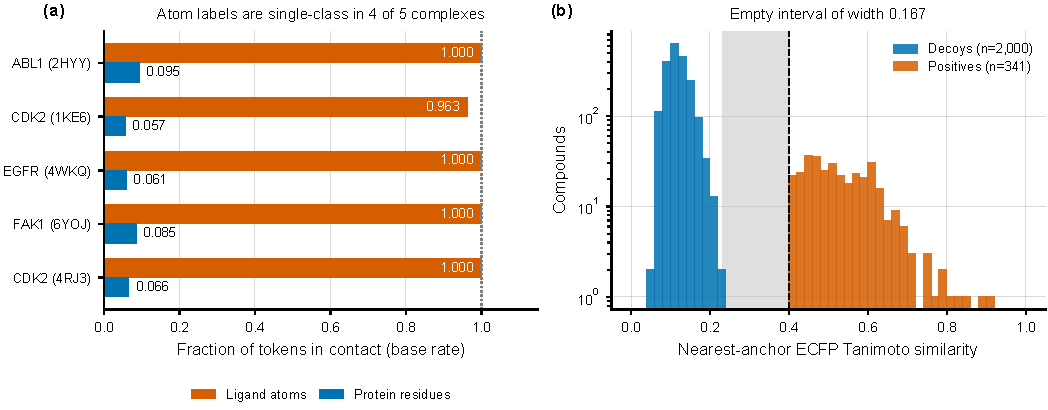
\includegraphics[width=\textwidth]{../results/fig_benchmark_validity.pdf}}%
{\fbox{Pending figure}}
\caption{Two benchmark constructions that prevent valid interpretation.
(a) Contact base rates in the five-complex kinase panel. Essentially every
ligand heavy atom is in contact, leaving a single-class label vector in four of
five complexes, while the residue-level base rate of 5.7\% to 9.5\% leaves a
well-posed problem. (b) Class-conditional nearest-anchor similarity for the
EGFR family panel. Positives were selected by requiring similarity $\geq 0.40$
to the reference binders from which the anchors were later drawn (dashed line);
decoys were sampled with no similarity constraint. The supports are disjoint,
separated by a shaded interval of width 0.167 containing no molecule of either
class, so no similarity-matched subpanel can be drawn and the comparison cannot
be repaired by reweighting.}
\label{fig:validity}
\end{figure*}

%% ------------------------------------------------------------------
\section{Discussion}
%% ------------------------------------------------------------------

\subsection{What the System Supports}
Auditing the secondary capabilities as strictly as the primary one leaves a
narrower but clearer recommendation.

\textbf{Supported: ranking within the evaluated chemical space.} Pooled
concordance index 0.8625 and AUROC 0.9240 support prioritization on the tested
KIBA pairs, but do not establish ranking accuracy within individual target
series. Limits of agreement span $-0.895$ to $0.876$ KIBA units, limiting
single-compound interpretation. The split contains no unseen compound or
target, so these results describe interpolation within known chemical space.

\textbf{Supported: interaction maps as a target-associated readout.} The map comes
from the same forward pass as the prediction and carries ligand-specific
information a linear probe recovers, but the shared residue profile accounts
for 92.7\% of its variance on the EGFR panel. Contact localization remains uncertain at the panel level.

\textbf{Potential use: screening without a reference active set.} The model outranks
AutoDock Vina by 0.188 AUROC and scores a candidate in 210\,ms against a median
of 104\,s per ligand for docking, on a workstation without an accelerator. Where a target has a
structure but no known actives, this motivates evaluation of a learned scorer;
performance on previously unseen targets remains unestablished.

\textbf{Not supported: prioritizing a library in preference to a similarity
search.} On the evaluated panels, a fingerprint search using known actives
leads the model by 0.156 AUROC in domain and also performs better out of domain.

\textbf{Partially supported: proposing follow-up chemistry.} The diffusion head
produces the lowest median fingerprint similarity to the seed among the three
generators, and 55 of its 56 audited proposals have lower docking scores than
the seed. However, it has no
yield advantage over fragment swaps, fewer than half its molecules pass the
Lipinski rules against 94\% for fragment swaps, every proposal shares the seed's
generic framework, and 4 of 60 could not be prepared for docking. As a
substitution enumerator it works; as a source of chemical novelty it is
unevidenced.

\subsection{Limitations}
The structural panel has five complexes across four targets, including two
CDK2 complexes, which limits target-level independence. Its variance components put the
requirement at 18 to 21 complexes to separate a residue contact AUROC of 0.585
from chance at 80\% power, against an estimated 0.20 to 0.30 under the assumed
effect and variance. These estimates assume independent complexes and do not include uncertainty
in the effect size or variance components.

Except for the archived three-seed ablations, analyses use one checkpoint and
one training seed. The component ablation cannot be strengthened
without retraining at a scale we did not run.

The retrieval comparisons are limited differently. H1 is out of domain, so it
tests transfer, and DUD-E's decoy selection may favor the fingerprint baseline
in domain, as discussed in Section~\ref{sec:retrieval}. The docking
reference used Open Babel receptor preparation and a single rigid conformation,
so it is a reference point rather than an optimized campaign.

Finally, both failure modes were characterized in panels we built, which is what
lets each be traced to a construction step. The literature audit extends the
first reporting gap to published work, without establishing saturation in those
studies; the prevalence of the second failure remains open.

%% ------------------------------------------------------------------
\section{Conclusion}
%% ------------------------------------------------------------------
We presented DeepDTA-iBAM, a multi-task architecture in which bidirectional
cross-attention between ligand atoms and protein residues supports affinity
prediction, interaction-map extraction, and retrieval. Analog generation shares
the protein adapter and checkpoint. The design claim is an interface
claim rather than an accuracy claim, and we measured it: the map is a byproduct
of the forward pass that yields the prediction. Retaining it had a measured
mean collection overhead of 1.5\%.

Auditing the secondary capabilities as strictly as the primary one is the second
half of the contribution. EGFR maps share a dominant residue profile but carry a
ligand-specific component from which a linear readout predicts part of the
predicted affinity and distinguishes active--decoy labels, including for compounds with no
crystal pose. Retraining ablations cannot single out any one component, though
disabling the fusion pathway increases the trained
model's RMSE by 33\%, and at retrieval the model outranks an established docking
program but trails a nearest-active fingerprint search.

Two benchmark constructions examined here prevent valid interpretation, and
three reporting checks detect both with minimal additional computation, separating a
benchmark that can be repaired from one that must be rebuilt. The path forward
is a matched follow-up in one target family: assay-defined positives with
property-matched decoys and no topological constraint
\cite{mysinger2012dude,trannguyen2020litpcba}, a larger co-crystal panel with verified structural annotations, and orthogonal scoring of generated compounds
\cite{vamathevan2019ml,stokes2020antibiotic}.

%% ------------------------------------------------------------------
\section*{Acknowledgment}
The authors thank the University of Alabama at Birmingham IT Research Computing
group for high-performance computing support and CPU and GPU time on the Cheaha
compute cluster, which was used for model training and evaluation.

\bibliographystyle{IEEEtran}
\bibliography{references}

%% ------------------------------------------------------------------
%% Author biographies
%%
%% Photoless biographies are accepted by IEEE Access; to include portraits,
%% swap IEEEbiographynophoto for IEEEbiography and supply the image files.
%% ------------------------------------------------------------------
\begin{IEEEbiographynophoto}{Kevin Song}
received the B.S. degree in biology and the M.S. degree in biomedical
informatics from Stanford University, Stanford, CA, USA. He is currently
pursuing the Ph.D. degree in biomedical engineering, with a concentration in
bioinformatics, at the University of Alabama at Birmingham (UAB), Birmingham,
AL, USA. His research brings together artificial intelligence, cheminformatics,
bioinformatics, and experimental biology, applied to drug discovery and to
cardiovascular regeneration.
\end{IEEEbiographynophoto}

\begin{IEEEbiographynophoto}{John Zhang}
received the B.S. degree in chemistry from the University of Minnesota,
Minneapolis, MN, USA, and the Master of Bioscience degree from Keck Graduate
Institute, Claremont, CA, USA. He is currently pursuing the Ph.D. degree in
biomedical engineering at UAB. His research focuses on cardiovascular
translational science, ischemic vascular dysfunction, cardiometabolic
signaling, and regenerative therapies.
\end{IEEEbiographynophoto}

\begin{IEEEbiographynophoto}{Lei Ye}
received the M.D. degree from Shanghai Medical University, Shanghai, China, and
the Ph.D. degree in biomedical science from the National University of
Singapore, Singapore. He is currently an Associate Professor of biomedical
engineering with UAB. His research focuses on cardiac tissue engineering, stem
cell biology, gene and cell therapy, and cardiovascular regeneration.
\end{IEEEbiographynophoto}

\begin{IEEEbiographynophoto}{Jianyi ``Jay'' Zhang}
received the M.D. degree from Shanghai Medical University, Shanghai, China, and
the Ph.D. degree in biomedical engineering from the University of Minnesota,
Minneapolis, MN, USA. He is currently a Distinguished Professor and the Chair
of biomedical engineering with UAB. His research focuses on cardiac tissue
engineering, myocardial bioenergetics, biomaterials, and stem-cell-based
cardiac repair.
\end{IEEEbiographynophoto}

\EOD
\end{document}
